%!TEX root = thesis.tex
\chapter{Background} \label{ch:background}

\todo[inline]{Lots more citations, preferably state that it's someone else's work, cite and then write about it.}

In this chapter, we introduce laser scanning and the 3D-reconstruction pipeline. In section~\ref{sec:heritage} we describe the heritage preservation context of this work. In section~\ref{sec:scanners} we introduce 3d scanning and describe the process by which raw scanner data transformed into a model in section~\ref{sec:pipeline}. This is then followed by a discussion the point cloud cleaning process in section~\ref{sec:cleaning}.


\section{Digital heritage preservation} \label{sec:heritage}

Architectural heritage sites in many parts of the world are under threat of destruction or deterioration, especially in developing countries. There is a need to preserve heritage sites due to their historical importance, if not physically, digitally. The demolition of  the Buddhas of Bamiyan by the Taliban in 2001 \cite{Toubekis2009} underlines the need for digital preservation efforts. Past preservation efforts have utilised many techniques to create a historical record of buildings and ruins. Early efforts made use of tape measures and theodolites to produce simple ground plans. \todo{Patrick need more general background: projects? other other todr? photo/text archiver? say why they are no longer used} More recently, photogrammetry lets geomaticians produce 3D models \cite{Heritage}. Laser range scanning is the latest technique that allows archivists to create extremely high resolution 3D models.

\todo{expand, say more, justify focus on laser scanning}

\section{3D scanning} \label{sec:scanners}

\todo[inline]{What is a range scanner, what is a point cloud, what is a range scan?}

There are many known types of 3D scanner on the market today. Each scanner has properties that make it more of less suitable for various scanning tasks. Generally, the size of the object and the level of detail one wishes to capture dictate the technology. Other factors like imaging speed, portability and cost or a scanner then comes into play.

3D Scanning technologies can generally be classified into 2 categories, namely triangulation and time of flight scanners.

\subsection{Triangulation scanners}

Triangulation scanners, as the name suggests, uses trigonometric triangulation \cite{Frohlich2004} to locate a point in a scene relative to the scanner. Triangulation scanners come in two flavors, those that use laser light and those that use white light \cite{Brown2012}. Laser scanners emit a laser pulse and records the reflected beam with a sensor at a known position relative to the laser. Light scanners emit a series of linear patterns that is also captured a sensor at a known position. The difference is that the sensor in the laser scanner directly measures the angle of the returned light where as the light sensors record perspective distortions in the reflected patterns to compute the angle of the returned light indirectly. Once the angle of incoming light is determined, the position of a far away point can be computed.

\begin{figure}[H]
	\begin{subfigure}[b]{.33\textwidth}
	  \centering
	  \includegraphics[width=.9\linewidth]{images/structured-light-scan}
	  \caption{}
	\end{subfigure}%
	\begin{subfigure}[b]{.33\textwidth}
	  \centering
	  \includegraphics[width=.9\linewidth]{images/triangulate-laser-scan}
	  \caption{}
	\end{subfigure}
	\begin{subfigure}[b]{.33\textwidth}
	  \centering
		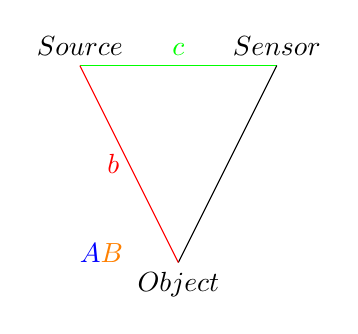
\begin{tikzpicture}[scale=2.5]

		\coordinate [label={[black]above:$Source$}] (A) at (0, 1);
		\coordinate [label={[black]above:$Sensor$}] (B) at (1, 1);
		\coordinate [label={[black]below:$Object$}] (C) at (0.5, 0);

		\draw[green] (A) -- node [above] {$c$} (B);
		\draw[black] (B) -- node [right] {$ $} (C);
		\draw[red] (C) -- node [left] {$b$} (A);

		\tkzMarkAngle[fill=white, size=0.25cm,%
		opacity=1](C,A,B)
		\tkzLabelAngle[pos=0.15](C,A,B){$\color{blue}A$}

		\tkzMarkAngle[fill=white,size=0.25cm,%
		opacity=1](A,B,C)
		\tkzLabelAngle[pos=-0.15](C,B,A){$\color{orange}B$}

		% \tkzMarkAngle[fill=green,size=0.25cm,%
		% opacity=.4](B,C,A)
		% \tkzLabelAngle[pos= 0.15](B,C,A){$ $}

		\end{tikzpicture}
		\caption{}
	\end{subfigure}
	\caption{Triangulation 3D scanners \protect\footnotemark}
	\label{fig:triangulation-scanners}
\end{figure}

Given the precise distance between the light source and sensor ($\begingroup\color{green}c\endgroup$) and as well as the outgoing angle of emitted light ($\begingroup\color{blue}A\endgroup$) and incoming angle of reflected light ($\begingroup\color{orange}B\endgroup$), the distance to the object is given by $\begingroup\color{red}b\endgroup = \begingroup\color{green}c\endgroup\frac{ sin(\begingroup\color{orange}B\endgroup)}{sin(\pi - \begingroup\color{blue}A\endgroup-\begingroup\color{orange}B\endgroup)}$.

\subsection{Time of flight scanners (TOF)} \label{subsec:tof}

\begin{figure}[ht]
  \centering
  \includegraphics[width=.5\linewidth]{images/pulse-tof}
  \caption[Time of flight scanner]{Time of flight scanner \protect\footnotemark[\value{footnote}]}
  \label{fig:tof}
\end{figure}
\footnotetext{Source: \url{http://www.rapidform.com/3d-scanners/}}

Time of flight scanners emit laser pulses and measure the time it takes for a pulse reflection to be detected by the scanner's sensor (see \autoref{fig:tof}). Given the speed of light, the distance traveled by the pulse can be determined. Given the time it takes for a pulses to travel to a surface and back to the scanner ($t$), the distance ($d$) is given by $d = ct/2$ where $c$ is the speed of light. The accuracy of the distance calculation depends on how precisely time can be measured \cite{Form2014}.

\begin{figure}[ht]
	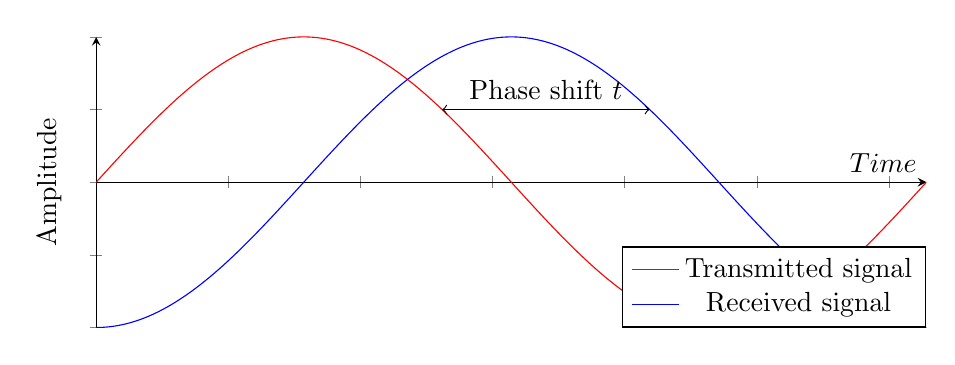
\begin{tikzpicture}[scale=1]
	\begin{axis}[
		width=1\textwidth,
		height=150,
	    axis lines = left,
	    yticklabels={,,},
	    xticklabels={,,},
	    axis x line=center,
	    xlabel = $Time$,
	    ylabel = {Amplitude},
	    legend style={
	    at={(1,0)},
	    anchor=south east}]
	]
	\addplot[samples=500,domain=0:2*pi, color=red]{sin(deg(x))};
	\addlegendentry{Transmitted signal}
	\addplot[samples=500,domain=0:2*pi, color=blue]{sin(deg(x-pi/2))};
	\addlegendentry{Received signal}
	\draw[<->] (axis cs:2.61799,0.5) -- node[above]{Phase shift $t$} (axis cs:4.18879,0.5);
	\end{axis}
	\end{tikzpicture}
	\caption{Phase shift in returned signal}
	\label{fig:phase-shift}
\end{figure}

Laser phase-shift scanners \cite{Frohlich2004} are a variation on the standard TOF scanner. These scanners modulate the power of the laser pulse in a sinusoidal wave during a scan. The phase shift in the returning pulse is used to compute the round trip time (see \autoref{fig:phase-shift}). Due to the cyclical nature of the signal, phase shift is ambiguous. This ambiguity is resolved by using measurements at multiple frequencies \cite{Bhurtha}.


\subsection{Comparison}

Triangulation scanners can achieve 10 micrometer accuracy over distances less than one meter. Over longer distances the triangle in \autoref{fig:triangulation-scanners} becomes elongated and the distance calculation error prone. Structured light scanners tend to be faster than laser scanners as the whole scene is captured instead of a single point at a time \cite{Brown2012}. Structured light scanners are also less prone to motion distortions. Hand held scanners of this type exists which reduces setup time compared to other scanners.

Time of flight scanners can measure the time a laser pulse takes to travel to and from an object very accurately over long distances. Pure TOF scanners can scan distances of up to 1000 meters \cite{Form2014}. TOF technology does not, however, deal well with distances less than 2 meters. Triangulation scanners on the other hand perform very well in the 2 meter range but suffers from accuracy issues beyond it. TOF scanners can be set to sample at different resolutions; low resolution scans (tens of thousands of points) may take seconds while higher resolution scans (millions of points) may take minutes.

Phase-based scanners have limited range due to the ambiguity of returned signals from beyond the design distance \cite{Bhurtha}; objects from beyond the scanner's designed range can sometimes be erroneously returned as closer distances when the scanner software fails to discard far away points. Phase based scanners make up for this deficiency by being much faster and more accurate within its range \cite{Form2014}.


\begin{table}
\begin{tabular}{ |l|l|l|l|l|l| }
  \hline
  Type &              Range &        Precision       & Speed & Portability \\
  \hline
  Structured light &    <1m     & 10 micrometer  & Seconds & High \\
  Laser triangulation & <1m     & 10 micrometer  & Seconds  & Medium \\     
  TOF &                 2-1000m & Medium      & Minutes & Low \\
  Phase &               2-100m & Low         & Seconds to Minutes & Low \\
  \hline  
\end{tabular}
\caption{Comparison of scanning technology}
\end{table}


\subsection{Data} \label{sec:data}

\footnotetext{Source: \url{http://www.rapidform.com/3d-scanners/}}

\begin{figure}[ht]
  \centering
  \includegraphics[width=1\linewidth]{images/grid}
  \caption{2D scan grid of intensity values \protect\footnotemark[\value{footnote}]}
  \label{fig:grid}
\end{figure}

\footnotetext{Rendering based on data provided by the \href{http://www.zamaniproject.org/}{Zamani Project}}


The terrestrial laser scanners described above all produce angle and range measurements that are converted into 3D coordinates relative to the scanner. Scanners also record the intensity of the light returned. High end scanners sometimes have integrated cameras that are used to map colors to captured data points \cite{Frohlich2004}. Data points are typically saved in 2D grid data structure (see \autoref{fig:grid}). Orientation and GPS measurements are also available in some models which help speed up registration (see \ref{sec:registration}).

Scanner manufacturers may also record lower level measurements that are specific to their scanners. This data may valuable in identifying artifacts from scans. Unfortunately, this data tends to be locked away in propriety formats which are not readily accessible. We therefore limit our investigation to data that can be readily exported from scanner software. We also do not consider color information as such datasets were not readily available for this work.

% (Mention non uniform point density somewhere? too obvious?)
% (Mention scanner resolution increasing over time?)

\subsection{Artifacts} \label{sec:artifacts}

In addition to the phase shifting issues (see \ref{subsec:tof}) which occur in phase-based TOF scanners, scanners are subject to a number of other limitations. Due to the optical nature of the described scanners, difficulties are often encountered when dealing with shiny, mirroring or transparent objects. Windows cannot be captured as light passes through without being reflected. Mirror-like surfaces are also missed because light does not reflect back towards the scanner. The sun and other bright objects and cause points not associated with any physical object to appear in a scan. Fog and smoke can also cause problems \cite{Ruther2011}.

\todo[inline]{More detail on artifacts}

\begin{figure}[ht]
  \centering
  \includegraphics[width=1\linewidth]{images/mixed-pixel}
  \caption{Mixed pixels. Green are valid points and red are not. \cite{Tuley2005}}
  \label{fig:mixed-pixel}
\end{figure}

Mixed pixels are another problematic aspect of laser scanning: when a laser pulse partially strikes a nearby and then, subsequently, a distant object, the result is a data point between the near and far object \cite{Tuley2005} (see \autoref{fig:mixed-pixel}).


Since time of flight scanners are generally used in the cultural heritage domain, because of their long range, these scanners will be the focus of our research. We thus limit ourselves to managing the artifacts introduced by such scanners when developing point processing algorithms.


\section{3D reconstruction pipeline} \label{sec:pipeline}


\begin{figure}

	% Define block styles
	\tikzstyle{decision} = [diamond, draw, fill=blue!20, 
	    text width=4.5em, text badly centered, node distance=3cm, inner sep=0pt]
	\tikzstyle{block} = [rectangle, draw, fill=gray!20, 
	    text width=5em, text centered, rounded corners, minimum height=4em]
	\tikzstyle{optionalblock} = [rectangle, draw, dashed,
	    text width=5em, text centered, rounded corners, minimum height=4em]
	\tikzstyle{line} = [draw, -latex']
	\tikzstyle{cloud} = [draw, ellipse,fill=red!20, node distance=3cm,
	    minimum height=2em]
	
	\centering

	\begin{tikzpicture}[node distance = 2cm, auto]
	    % Place nodes
	    \node [block] (acquire) {Scan acquisition};

	    \node [optionalblock, below right of=acquire, node distance=3cm] (clean) {\bf{Clean}};
	    \node [block, below left of=acquire, node distance=3cm] (register) {Register};
	    \node [block, below of=acquire, node distance=4cm] (reconstruct) {Reconstruct surface};
	    \node [optionalblock, right of=reconstruct, node distance=3cm] (autofill) {Automatic hole filling};
	    \node [optionalblock, left of=reconstruct, node distance=3cm] (filling) {Manual hole filling};
	    \node [block, below of=reconstruct, node distance=2cm] (texture) {Texture};
	    % Draw edges
	    \path [line] (acquire) -- (clean);
	    \path [line] (acquire) -- (register);
	    \path [line][<->] (clean) -- (register);
	    \path [line] (register) -- (reconstruct);
	    \path [line][-] (reconstruct) -- (autofill);
	    \path [line] (reconstruct) -- (filling);
	    \path [line] (filling) -- (texture);
	    \path [line] (reconstruct) -- (texture);

	    \draw[densely dotted] (1.7,-5.3) rectangle (4.7,-6.7);

	    % legend
	    \node [block, right of=texture, node distance=2.5cm, scale=0.7,
	    	text width=3.8em, minimum height=1em](required) {Required step};
	    \node [optionalblock, right of=required, node distance=1.4cm, scale=0.7,
	    	text width=3.8em, minimum height=1em] (notrequired) {Optional step};

	\end{tikzpicture}

	\caption{Reconstruction pipeline \protect\footnotemark[\value{footnote}]}
	\label{fig:pipeline}

\end{figure}
\footnotetext{Adapted from \cite{Ruther2011}}

3D reconstruction of a site starts with the acquisition of range scans in the field. The collection of raw scans are then subject to a series of processing steps. Unwanted objects and noise are typically removed and missing data can be synthesized. The scans then need to transformed to onto a common coordinate frame in a process called registration. A surface model can then be constructed from the registered point sets. The final model is complete when the reconstructed mesh is textured (see \autoref{fig:pipeline}) \cite{Ruther2011}.

\subsection{Data acquisition}
Some degree of planning is required to ensure the successful 3D reconstruction of a heritage site \cite{Ruther2011}. One needs to decide on an appropriate level of scan detail for different areas as the set resolution of a scanner determines the data acquisition rate. Scanner positions that result in flat angles of incidence with surfaces should be avoided to maximize surface detail. Choosing good scanning positions will ensure that maximum site coverage is achieved in the most economical way \cite{Ruther2011}.

Some additional considerations can speed up later steps in the pipeline. For example automated registration tools require requires that that overlap between scans are achieved. Positioning the scanner in the same level orientation also helps with registration \cite{Ruther2011}.

\subsection{Registration}  \label{sec:registration}

\begin{figure}[ht]
  \centering
  \includegraphics[width=0.6\linewidth]{images/registration}
  \caption{ICP correspondences \protect\footnotemark.}
  \label{fig:registration}
\end{figure}
\footnotetext{Source: \url{http://pointclouds.org/documentation/}}

Two approaches exist to transform all scans into a common coordinate system. The first approach requires placing reference objects, called targets, around a site during data acquisition. When the same object is found in two scans, the object's shape can be used to align the scans. The second approach, Iterated Closest Point (ICP) aligns scans by using surface features \cite{Besl1992}.

Automated software easily identify targets and provide highly accurate registration. Targets do, however, have to captured in high resolution in order to be useful. This may require one to capture more scans than required for simple documentation purposes. In the heritage domain targets have been found to be impractical as they often need to be placed in hard to reach places and intricate indoor environments require too many targets \cite{Ruther2011}. 

ICP requires less effort during data acquisition. However the registration procedure requires that two surfaces are roughly aligned as an initial condition, usually by hand. Correspondences are then computed between the surfaces where after an incremental transformation is computed to minimize the distance between all the correspondences. After the transformation is applied, the procedure is repeated until convergence is reached. There are many variations to the ICP algorithm that vary mainly on the type of correspondent matching and optimization procedure used \cite{Besl1992}.  

A user needs to ensure a good initial alignment or convergence may not be achieved. Featureless surfaces are also problematic as the optimization problem will have multiple solutions which may lead to misalignment.

\subsection{Cleaning}\label{sec:cleaning}

\begin{figure}[ht]
	\begin{subfigure}[b]{.5\textwidth}
	  \centering
	  \includegraphics[width=.9\linewidth]{images/dirty}
	  % \caption{Structured light 3D scanning \cite{Form2014}}
	  % \label{fig:structured-light-scan}
	\end{subfigure}%
	\begin{subfigure}[b]{.5\textwidth}
	  \centering
	  \includegraphics[width=.9\linewidth]{images/clean}
	  % \caption{Laser 3D scanning}
	  % \label{fig:images/triangulate-laser-scan}
	\end{subfigure}
  \caption{Trees cleaned from a scan}
  \label{fig:cleaning}
\end{figure}

Cleaning is considered an optional step for documentation purposes, however, neglecting it in the modeling pipeline can lead to poor results during surface reconstruction (see \autoref{sec:reconstruction}). Trees, people, cables, cars, doors, animals and other random unwanted objects, as well as scanner artifacts (\autoref{sec:artifacts}) are removed during the cleaning process. Cleaning can be performed on individual scans before registration or/and on the complete point cloud after registration \cite{Ruther2011}.

Cleaning one scan at a time requires less system resources and reduces the combined point cloud size. Unfortunately in some instances one may remove unwanted objects that are necessary for registering otherwise featureless surfaces. A tree on a flat surface could help the correspondence matching step in ICP that would otherwise not converge. One may therefore leave some unwanted objects that will have to be removed from the combined model. Range scans are may be hard to clean as the cleaner only gets to see objects from one perspective. Laser range scanners also produce point sets that have non uniform density: objects further away from the scanner are sampled less densely. It is thus harder to identify objects that are far away. Having an individual 2D scan grid allows one to view the 3D scan like a photograph (see \autoref{fig:grid}). This 2D perspective may disambiguate objects that are hard to identify in 3D. 

Registering all scans and combining them into a single point model destroys the embedded 2D grid structure and results in a large unorganized point cloud. With this transformation one loses the ability to perform constant time neighbour lookups via a grid. Neighborhood searches are important for normal estimation which is used during surface reconstruction. Without the scan grid, less efficient ($O(log(n))$) octrees or kd-trees are necessary for neighborhood searches. There is also an increased risk of estimating bad normals from merged data sets \cite{Ruther2011}. Alternatively one may choose to pre-compute point normals prior to merging data sets. This will however increase the file size.

Combining scans into a single point cloud does reduce the workload as overlapping areas only require a single cleaning pass. A complete model will typically be too large to fit into main memory and thus out-of-core techniques \todo{Explain, we do not address this} are required to manage the data sets.

Some heritage scanning projects have reported typical scans taking from 30 minutes up to 120 minutes to clean by an experienced person \cite{Ruther2011}. High resolution scans can take up to a full day to clean. Existing tools leave much to be desired in terms of cleaning efficiency. As cleaning is the part of the pipeline that is the focus of this work, more detail is presented in the next section.

\todo[inline]{software packages? Focus on accuracy}

\subsection{Surface reconstruction}  \label{sec:reconstruction}

% \begin{figure}[ht]
%   \centering
%   \includegraphics[width=0.6\linewidth]{images/mls}
%   \caption{Surface fitting \protect\footnotemark.}
%   \label{fig:registration}
% \end{figure}
% \footnotetext{Source: \url{http://en.wikipedia.org/wiki/File:Linear_regression.svg}}

Surface reconstruction is the process by which the discrete point model is converted to a triangulated surface model. This can be achieved either via interpolation methods, that aim to connect neighboring points by computing a triangulation, or by approximation methods that aim to approximate a surface that fits the samples \cite{Schall2005}.

Interpolation methods are very sensitive to noise. Poor triangulations are achieved when scans are not properly registered or the sampling exhibits high variance. A preprocessing can mitigate these problems but tends to be time consuming and often lead to a loss of detail \cite{Ruther2011}.

Surface approximation algorithms are less susceptible to noise. Poisson surface reconstruction \cite{Kazhdan2006} is a popular method that is noise resistant and achieves great detail. It uses samples with normals to interpolate a normal field and then solves a Poisson equation to compute an indicator function. Results are dependent on good normal estimations. It is thus preferable to compute normals prior to registration when using this approach. Poisson surface reconstruction produces ``water-tight'' surfaces and automatically fills small holes. While this is useful for producing a visually pleasing 3D model, it does not result in a historically accurate model because some data may be synthesized in the process.

Moving Least Squares (MLS) is another popular surface approximation method that does not over smooth and interpolate missing data \cite{Merry2014}. Like Poisson, it also requires normal estimates. MLS computes a local surface approximation at a sample point by considering its neighborhood. Every point in a neighborhood is weighed according to its importance. A surface is then computed by minimizing the weighed distance to the surface for each point in the neighborhood. Poisson and MLS have both been adapted for out-of-core execution and GPU acceleration \cite{Merry2014}. 


% This is especially problematic when working with individual scans as the sampling density reduces away from the scan origin.


% When parameters are set to exclude or filter questionable data, there is a higher likelihood of holes in t


\subsection{Hole filling} \label{sec:filling}

It is unlikely that a scanning expedition will achieve complete coverage of a site. Furthermore, points are removed during cleaning and reconstruction of the surface. Hole filling is an optional step in the reconstruction pipeline that seeks to synthesis missing data. For historical accuracy, hole filling is not desirable since data is synthesized. However, models that have been filled are more aesthetically pleasing. If holes are filled it is thus important to know what data has been synthesized.

Small holes can be filled automatically by surface reconstruction algorithms (as discussed above). Larger patches are hard to fill convincingly with automated methods and may require manual effort to produce good results \cite{Ruther2011}. 

\todo{ask patrick for citations}

\subsection{Texturing} \label{sec:texturing}

The final, optional, step of the reconstruction pipeline is texturing. Coloring a model is not only visually pleasing but also forms part of the historical record. Some laser scanners come equipped with cameras to capture color information for each sample. Although this is very convenient, some in the heritage community have reported that poor texturing is achieved when compared to external cameras \cite{Ruther2011}. The biggest problem when texturing a model is dealing with different light conditions during the day. Capturing photos around the same time of day across multiple days is one way to mitigate the problem.

A model is textured from a series of photos by projecting the images onto the model. In order to achieve this, internal and external camera parameters needs to be known from time the picture is taken. This includes the position and orientation of the camera as well as the focal length. If this is not known it can be estimated via software by selecting or computing correspondences between pictures \cite{Ruther2011}.

\todo{more citations on texturing, ask rudy}


% \section{Point cloud cleaning} \label{sec:cleaning}
% 	Focused specifically on the task of point cloud cleaning in heritage scenes

% 	\subsection{Problem}
% 	Characterize heritage scenes
% 	\begin{itemize}
% 		\item Large scans
% 		\item many scans
% 		\item Non uniform density
% 		\item Large point sets
% 		\item Hard to distinguish trees from walls
% 	\end{itemize}

% 	\subsection{Existing systems}
% 		\begin{itemize}
% 			\item Z\&Y
% 			\item Cyclone
% 			\item Pointools
% 			\item Meshlab
% 			\item VR Mesh Studio
% 			\item Carlson Pointcloud
% 			\item 3D Reshaper
% 			\item Terrascan
% 		\end{itemize}

% 	\subsection{Evaluation of existing systems}
% 	We should look at existing systems in terms of a testing framework
% 	Evaluate their tools
% 	Evaluate user interface
% 	\begin{itemize}
% 		\item navigation: camera vs object move
% 		\item tool set (what tools are available)
% 		\item license
% 		\item 2d/3d editing
% 		\item extensibility (why did I not use it)
% 	\end{itemize}

		

% \section{Summary}
% %What do I conclude from all this and lead into the next chapter.	



% \section{Review of literature}

% \cite{Spina2010} Cultural heritage segmentation

